\documentclass{beamer}

% theme
\usetheme[sectionsymbol=$\circ$]{ModusPonens}
\usefonttheme{Electric}
\usecolortheme{Electric}

\usepackage[utf8]{inputenc}
\usepackage{graphicx} % Allows including images

% English date
\usepackage[english]{babel}

% tikz
\usepackage{tikz}
\usetikzlibrary{shapes,positioning}

\tikzstyle{vertex}=[draw, circle, inner sep=0pt, minimum size=8pt, fill=white, thick]
\tikzstyle{edge}=[rounded corners, draw=black, very thick]
\tikzstyle{lookhere}=[draw=red, circle, inner sep=0pt, minimum size=7pt, fill=none, very thick]

%----------------------------------------------------------------------------------------
%	TITLE PAGE
%----------------------------------------------------------------------------------------

\title[]{This Is The Title\\Of My Presentation}
\subtitle{It's Quite Interesting}
\author[Me]{Emma Example}
\titlenote{Joint work with Me and Myself}
\institute[]{University of Osnabrück}
% \logo{\includegraphics[height=1.9cm]{logo-small.png}}
\email{xyz@mail.com}

\date{\today}
%-----------------------------------------------------------------------------------------
\begin{document}

\begin{frame}
    \titlepage
\end{frame}

\begin{frame}
    \frametitle{Overview}
    \tableofcontents
\end{frame}

\section{Important Section 1}
\begin{frame}
    \frametitle{Title}
    \begin{block}{}
        \textbf{1:} Yes\\
        \textbf{2:} No
    \end{block}

    \begin{center}
        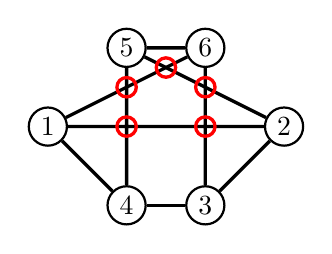
\begin{tikzpicture}[scale=1]
            \begin{scope}[every node/.style={vertex,inner sep=2pt}]
                \node (1) at (0,1) {1};
                \node (2) at (3,1) {2};
                \node (3) at (2,0) {3};
                \node (4) at (1,0) {4};
                \node (5) at (1,2) {5};
                \node (6) at (2,2) {6};
            \end{scope}

            \begin{scope}[every path/.style={edge}]
                \path (1) -- (2) -- (3) -- (6) -- (5) -- (4) -- (1);
                \path (2) -- (5);
                \path (4) -- (3);
                \path (6) -- (1);
            \end{scope}

            \begin{scope}[every node/.style={lookhere}]
                \node (c1) at (1,1) {};
                \node (c2) at (2,1) {};
                \node (c3) at (1,1.5) {};
                \node (c4) at (2,1.5) {};
                \node (c5) at (1.5,1.75) {};
            \end{scope}
        \end{tikzpicture}%
        \qquad\qquad%\pause%
        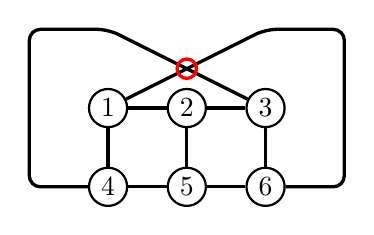
\begin{tikzpicture}[scale=1]
            \begin{scope}[every node/.style={vertex,inner sep=2pt}]
                \node (1) at (0,1) {1};
                \node (2) at (1,1) {2};
                \node (3) at (2,1) {3};
                \node (4) at (0,0) {4};
                \node (5) at (1,0) {5};
                \node (6) at (2,0) {6};
            \end{scope}

            \begin{scope}[every path/.style={edge}]
                \path (1) -- (2) -- (3) -- (6) -- (5) -- (4) -- (1);
                \path (2) -- (5);
                \path (4) -- (-1,0) -- (-1,2) -- (0,2) -- (3);
                \path (6) -- (3,0) -- (3,2) -- (2,2) -- (1);
            \end{scope}

            \begin{scope}[every node/.style={lookhere}]
                \node (c1) at (1,1.5) {};
            \end{scope}
        \end{tikzpicture}
    \end{center}
\end{frame}


\section{Important Section 2}
\subsection{Subsection}
\begin{frame}
    \frametitle{Title}
    \framesubtitle{Subtitle}
    \begin{itemize}
        \item Item 1
        \item Item 2
    \end{itemize}
    \bigskip

    \begin{enumerate}
        \item Item 1
        \item Item 2
    \end{enumerate}
\end{frame}

\section{Less Important Section 3}
\begin{frame}
    \frametitle{This is another frame}
    \begin{center}
        Example text here!
    \end{center}
\end{frame}

\section{Great Conclusion: Section 4}
% \section{Extra: Special Section 5}
\begin{frame}[noframenumbering]
    \frametitle{No Frame Number}
    \begin{center}
        \Huge Example text here!
    \end{center}
\end{frame}

\end{document}
